\documentclass{ctexart}
\usepackage{graphicx}
\usepackage{caption}
\usepackage{float}
\usepackage{amsmath}
\usepackage{fancyhdr}
\usepackage{xunicode-addon}
\usepackage{booktabs}
\usepackage{listings}
\usepackage{hyperref}
\usepackage[a4paper,hmargin=1.25in,vmargin=1in]{geometry}
% !TeX program = xelatex
\lstdefinestyle{mystyle}{
  basicstyle=\ttfamily\footnotesize,
  breakatwhitespace=false,         
  breaklines=true,                 
  captionpos=b,                    
  keepspaces=true,                 
  numbers=left,                    
  numbersep=5pt,                  
  showspaces=false,                
  showstringspaces=false,
  showtabs=false,                  
  tabsize=2
}

\lstset{style=mystyle}

\title{\begin{figure}[H]
	\centering 
	\includegraphics[height=7cm,width=14cm]{E:/Pictures/中科大.jpg}
	\end{figure}\Huge\textbf{人工智能原理与技术}\\\huge{实验4}}
\date{}
\punctstyle{banjiao} 
\pagestyle{fancy}
	\fancyhead[C]{\LARGE\textbf{实验4}}
	\fancyhead[L]{}
	\fancyhead[R]{}
	\fancyfoot[C]{\thepage}
\begin{document}
	\maketitle
	\thispagestyle{empty}
	
	\[\makebox{\Large{姓名:\underline{\makebox[5cm]{高茂航}}}}\]
	
    \[\makebox{\Large{学号:\underline{\makebox[5cm]{PB22061161}}}}\]
	
	$$\makebox{\Large{日期:\underline{\makebox[5cm]{2024.7.6}}}}$$
	
	\clearpage

	\pagenumbering{arabic}

	\section{Torch配置}

	\begin{figure}[H]
		\centering 
		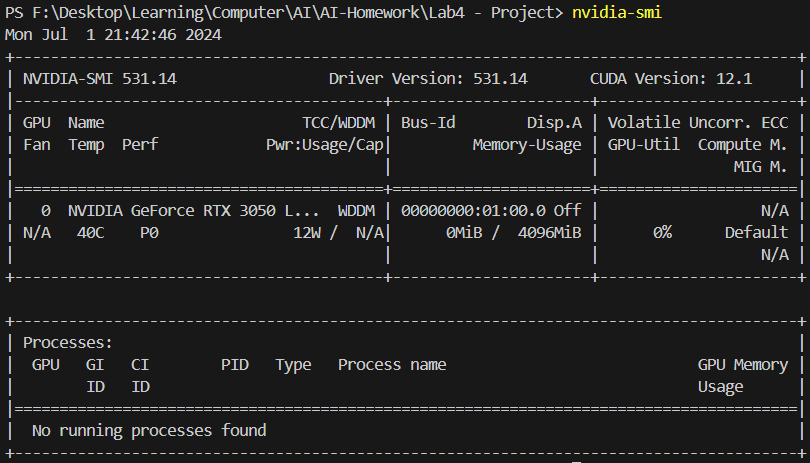
\includegraphics[height=5.5cm,width=10cm]{1.png}
		\end{figure}
		\begin{figure}[H]
			\centering 
			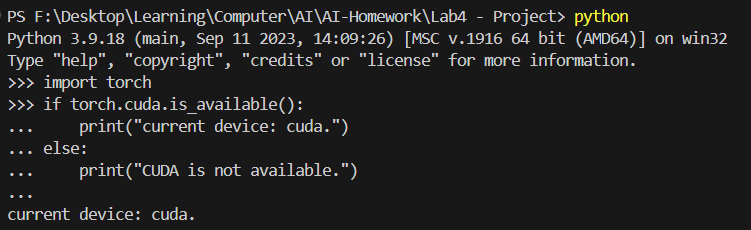
\includegraphics[height=3cm,width=10cm]{2.png}
			\end{figure}
	
	\section{实验原理}
\subsection{二元零和马尔可夫博弈}
一个涉及两个玩家在一系列状态中进行决策的过程,其中每个玩家的目标是最大化自己的累计奖励(或最小化对方的累计奖励),而这个过程的状态转移遵循马尔可夫性质。
在每个状态,玩家需要基于当前的信息选择最优策略,而这个选择会影响到游戏的下一个状态和玩家的即时奖励。由于是零和博弈,一个玩家的收益等于另一个玩家的损失,使得这种博弈具有高度的竞争性。
\subsection{Naive Self Play}
让AI与其自身的副本进行对战,通过这种方式根据自身经验不断学习适应并调整,以提高其性能。该方法较为简单直接,如果要避免不收敛等问题,需要采取更复杂的算法。
\subsection{Actor-Critic}
这种方法旨在通过同时学习一个策略(即Actor)和一个值函数(即Critic)来平衡探索和利用,从而提高学习效率和性能。
Actor根据当前策略选择动作,并执行该动作。Critic评估执行动作后的结果,即计算实际回报与预期回报之间的差异(TD误差)。
接着使用TD误差来更新Critic的值函数参数,使其预测更加准确。
最后根据Critic提供的反馈(TD误差),更新Actor的策略参数,以便在未来选择更好的动作。
	\section{constrained policy的解决思路}
	\section{optimize函数中3个bug的的解决方案}
	\section{其他bug及解决方案}
	\section{难以理解的点及解释}
	\section{loss 和 entropy 曲线分析}
	\section{}
	\section{}
	\section{课程反馈}



	

\end{document}